\justifying

\section*{\textbf{Exercise 1: From failure cause to outage}}
\begin{enumerate}
    \item weather conditions (snow/ice on transmission lines and wind) - failure cause
    \item mechanical wear of conductor by line dancing - failure mechanism
    \item broken conductor of an overheard fault - failure mode 
    \item short circuit (line-ground) - fault
    \item switched off automatically - outage
\end{enumerate}

\section*{\textbf{Exercise 2: failure causes line/cables}}
%Devendra
\begin{itemize}
    \item From the graphs provided for the causes of failure in overhead line and underground cables we see that external factors are the maximum contributing factor in the failure of overhead lines whereas excavation/hoisting work is the maximum contributing factor in the failure of underground cables. 
    \item One key difference in the two graphs is that the overhead lines are affected significantly due to weather effects such as wind, snow, hail etc. This is not the case for underground cables as they are protected from such environmental conditions.
    \item The underground cables are prone to wearing and aging as it is difficult to continually check up on the health of the cable due to it being underneath the ground. There is also an added possibility of failure during excavation to asses the aging of the cable. This is least contributing factor in overhead lines as it is easy to asses and act on the aging of the line since its not concealed.
\end{itemize}


\section*{\textbf{Exercise 3: large blackouts of power systems}}
%Devendra
\begin{itemize}
    \item Rank 1 is a cascaded failure: the second disconnector's arching was caused because the first disconnector was not closed successfully
    \item Rank 2 is a common cause and failure due to other complicating factors. The helicopter destroying the circuits in the transmission is a common cause whereas the delay in repair (since the lines were over a river) is categorized as other complicating factors
    \item Rank 3 is common cause and cascading. The gas leakage causes failure of multiple components (rail and transformer and protection malfunctioning of 2nd transformer), therefore it is a common cause. Whereas, the protection failure of the 2nd transformer caused overloading of the 3rd one which is a cascading failure
    \item Rank 4 is a cascading failure since the disconnection of a transformer caused fire which caused the complete installation to be switched off.
    \item Rank 5 is common cause since a short circuit caused fire and destroyed the complete installation
    \item Rank 6 is a combination of failures due to other complicating factors and common cause
    \item Rank 7 is a cascaded failure exploding of the transformer caused the protection system to fail which caused the entire station to be turned off
    \item Rank 8 is a cascaded failure since incorrect switching off of one transformer caused the overloading of another transformer
    \item Rank 9 is a common cause failure since an earth fault caused multiple component failure
    \item Rank 10 is a common cause since a common factor (boat) caused the failure
\end{itemize}
\section*{\textbf{Exercise 4: component (un)availability}}
%Saumitra
Unavailability is defined as the porbability that a component is under repair for a arbitrary time. It is the ratio of Repair time and Mean time between failures.
 The following table gives the unavailability of all the components mentioned in exercise 4 :

\begin{table}[H]
    \centering
    \begin{tabular}{lcccc}
         \multicolumn{1}{c}{\textbf{Component}} & \textbf{Failure Frequency} & \textbf{\begin{tabular}[c]{@{}c@{}}Mean Time\\  between \\ Failures\end{tabular}} & \textbf{\begin{tabular}[c]{@{}c@{}}Repair Time\\ (hrs)\end{tabular}} & \textbf{\begin{tabular}[c]{@{}c@{}}Unavailability\\ (hrs/year)\end{tabular}} \\
10 km HV overhead line                & 0.0051                     & 19.60784                                                                          & 8                                                                    & 0.4080                                                                       \\
10 km cable with joints               & 0.0284                     & 34.4828                                                                           & 249                                                                  & 7.214                                                                        \\
EHV Onshore Transformer               & 0.039                      & 25.641                                                                            & 23                                                                   & 0.88                                                                         \\
Converter Transformer                 & 0.037                      & 1580                                                                              & 1580                                                                 & 58.47                       
    \end{tabular}
    \caption{Unavailability of Components}
    \label{tab:my_label}
\end{table}
The differences can be observed in overhead line and underground cable. It is quite obvious, because of different probability of faults in both cases. Even if the faults occurring is the same, underground cable will take more time for repair and maintenance. This in-turn will increase its unavailability significantly.\par
Similarly, both the transformers depict different values for unavailability, with converter transformer having a larger unavailability. This is because it goes under a heavier wear and tear due to its location. Plus addition of power electronic components involves more intricate maintenance and repair.
\section*{\textbf{Exercise 5: offshore wind farm}}
%Saumitra
\begin{itemize}
    \item  The installed capacity of the Off-shore wind power plant is 350 MW.
    \item  Total Energy Generated is given by :
     \begin{equation}
         Total \,Energy\, Generation = Average \,Energy\, generated\, per\, year \times 8736
     \end{equation}
     Energy generated per year by the offshore wind power plant is 1386.7 Gwh.
    \item Capcity factor is given by :
    
    \[Capacity Factor =\frac{Actual Energy Generated}{Total Energy Generated}\]
    
     
    Capacity factor of this wind farm is 0.4535.
    \item The capacity factor of an on-shore wind farm will be less than off-shore. This is because the wind speeds are less on-shore as compared to off-shore which lead to a lower actual generation.
    \item The Power Duration Curve (PDC) is as follows :
    \begin{figure}[H]
        \centering
        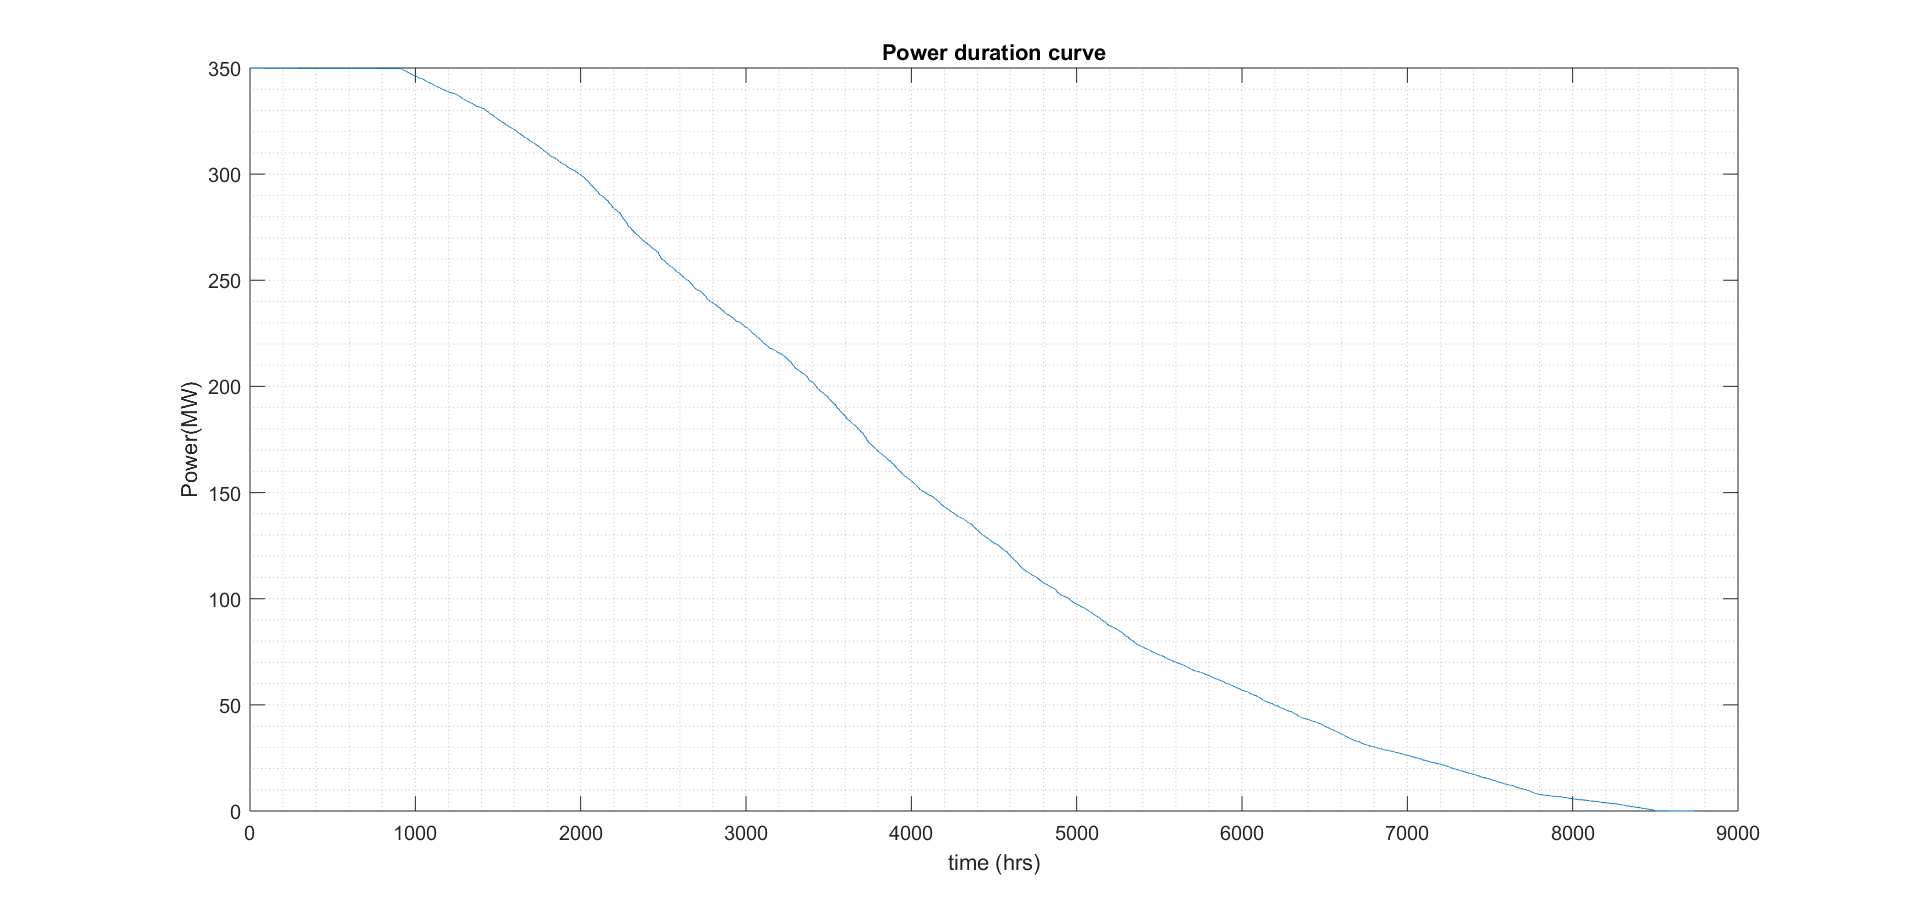
\includegraphics[width=0.8 \linewidth]{PDC_Q6.png}
        \caption{Power Duration Curve of Off-shore wind plant}
        \label{fig:my_label}
    \end{figure}
\end{itemize}
\section*{\textbf{Exercise 6: offshore wind farm connection 1}}
\begin{figure}[H]
\centering
        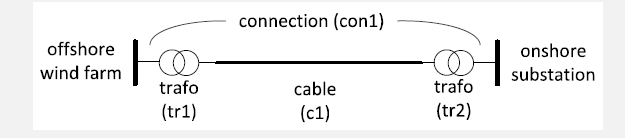
\includegraphics[width=0.8 \linewidth]{Q6_circuit1.PNG}
        \caption{Circuit diagram for single bus}
        \label{fig:circuit_label}
    \end{figure}
The given circuit has 3 components in series and the uncertainties are found in the following way:
\begin{equation}
         P(unavailitbility)=\frac{Repair time(h)}{8760}*frqeuency 
         \label{eq:uequation}
     \end{equation}
\begin{table}[htbp]
  \centering
  \caption{Uncertainties of components}
    \begin{tabular}{|r|r|r|}
    \hline
    \multicolumn{1}{|l|}{Cable} & \multicolumn{1}{p{5.415em}|}{Offshore transformer} & \multicolumn{1}{p{5.79em}|}{Onshore transformer} \bigstrut\\
    \hline
    0.001161 & 0.00667352 & 0.000102397 \bigstrut\\
    \hline
    \end{tabular}%
  \label{eq:uncertties}%
\end{table}%
The uncertainties of all components are calculated as per equation \ref{eq:uequation} and are tabulated in table \ref{eq:uncertties}
To calculate the total unavailability in case 1 where only one bus is present the equation stated below is
\begin{equation}
         P(A\cup B \cup C)= P(A)+P(B)+P(C)-P(A\cap B)-P(B\cap C)-P(A\cap C)+P(A \cap B\cap C \cap D)
         
\end{equation}
    
We get 69.77 hours on unavailability in this case, to find energy that is lost is we multiply the area under the curve of PDC and it is multiplied with the total uncertainty: 10.99 GWh and that is 0.79\% of energy that is lost.
\begin{figure}
    \centering
        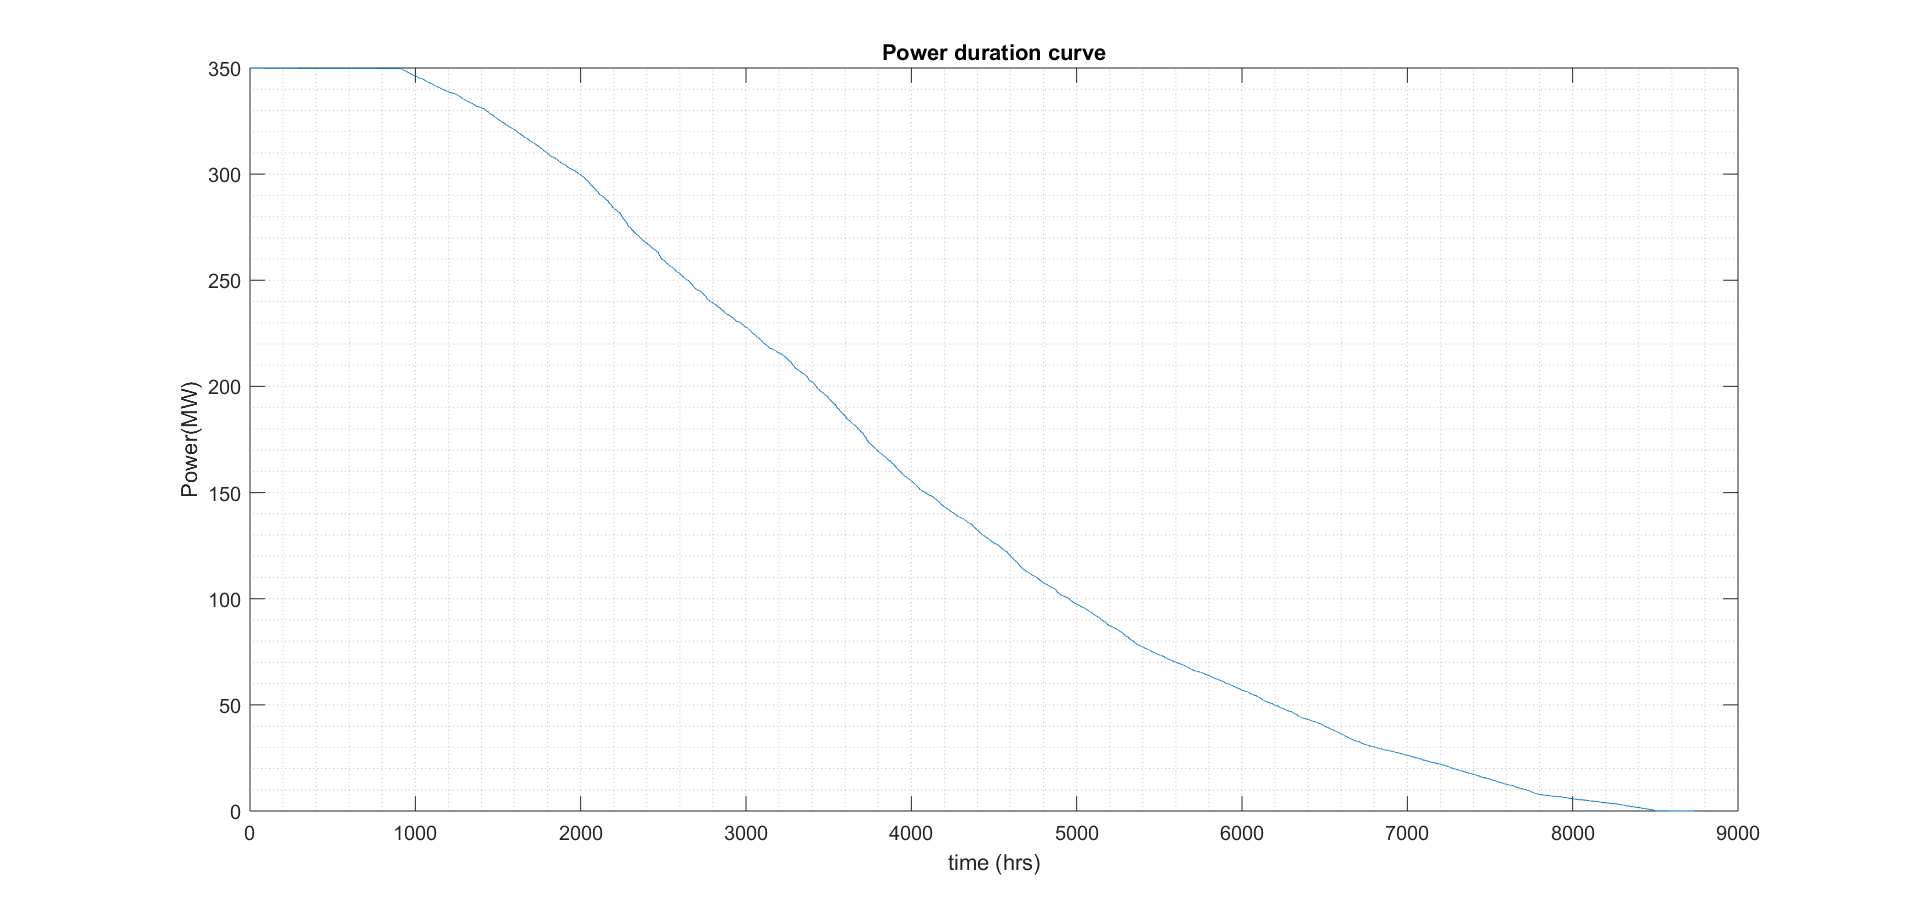
\includegraphics[width=0.8 \linewidth]{PDC_Q6.png}
        \caption{PDC of single bus}
        \label{fig:PDC for single bus}
\end{figure}
In the case with two buses there can be 3 major possibilities :\\
(0,0):both unavailable\\
(1,0) or (0,1): one available
(1,1): Both available

When there are two buses the worst case is when 2 lines are unavailable but the probability of that event is 0.00006525 hence the case where one just one bus fails is 0.015 and hence we consider that for energy that is lost and hence 13.62 GWh is lost and it is 0.49\% of the total energy. The energy that is lost is technically calculated from the PDC by drawing an horizontal line at P=350 MW and then taking the area above it. 

     
     
%\begin{table}[htbp]


%Omkar

\section*{\textbf{Exercise 7: offshore wind farm connection 2}}
In the given question the system is analyzed with and without coupler 
\begin{figure}[h!]
    \centering
        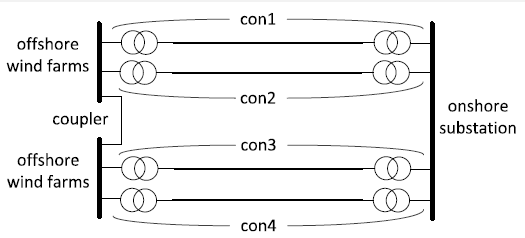
\includegraphics[width=0.8 \linewidth]{Coupler.PNG}
        \caption{Coupled and non coupled circuit}
        \label{fig:coupler}
\end{figure}
In the case where there is no coupler, two systems consisting of two buses in parallel are inturn in series with each other.\\
This leads to 4 possible failure cases\\
(0,0,0,0): all unavailable\\
(1,0,1,0) and the other combinations\\
(1,1,0,0) and all combinations\\
(1,1,1,0) and all combination\\
For the design usually the worst case scenario must be considered and here we find that the probability of 4 lines failing together is higher with a probability of 0.031 and this leads to an energy loss of 17.3 GWh and it is about 0.31\% of the total. The energy is obtained from the graph shown below.
\begin{figure}[h!]
    \centering
        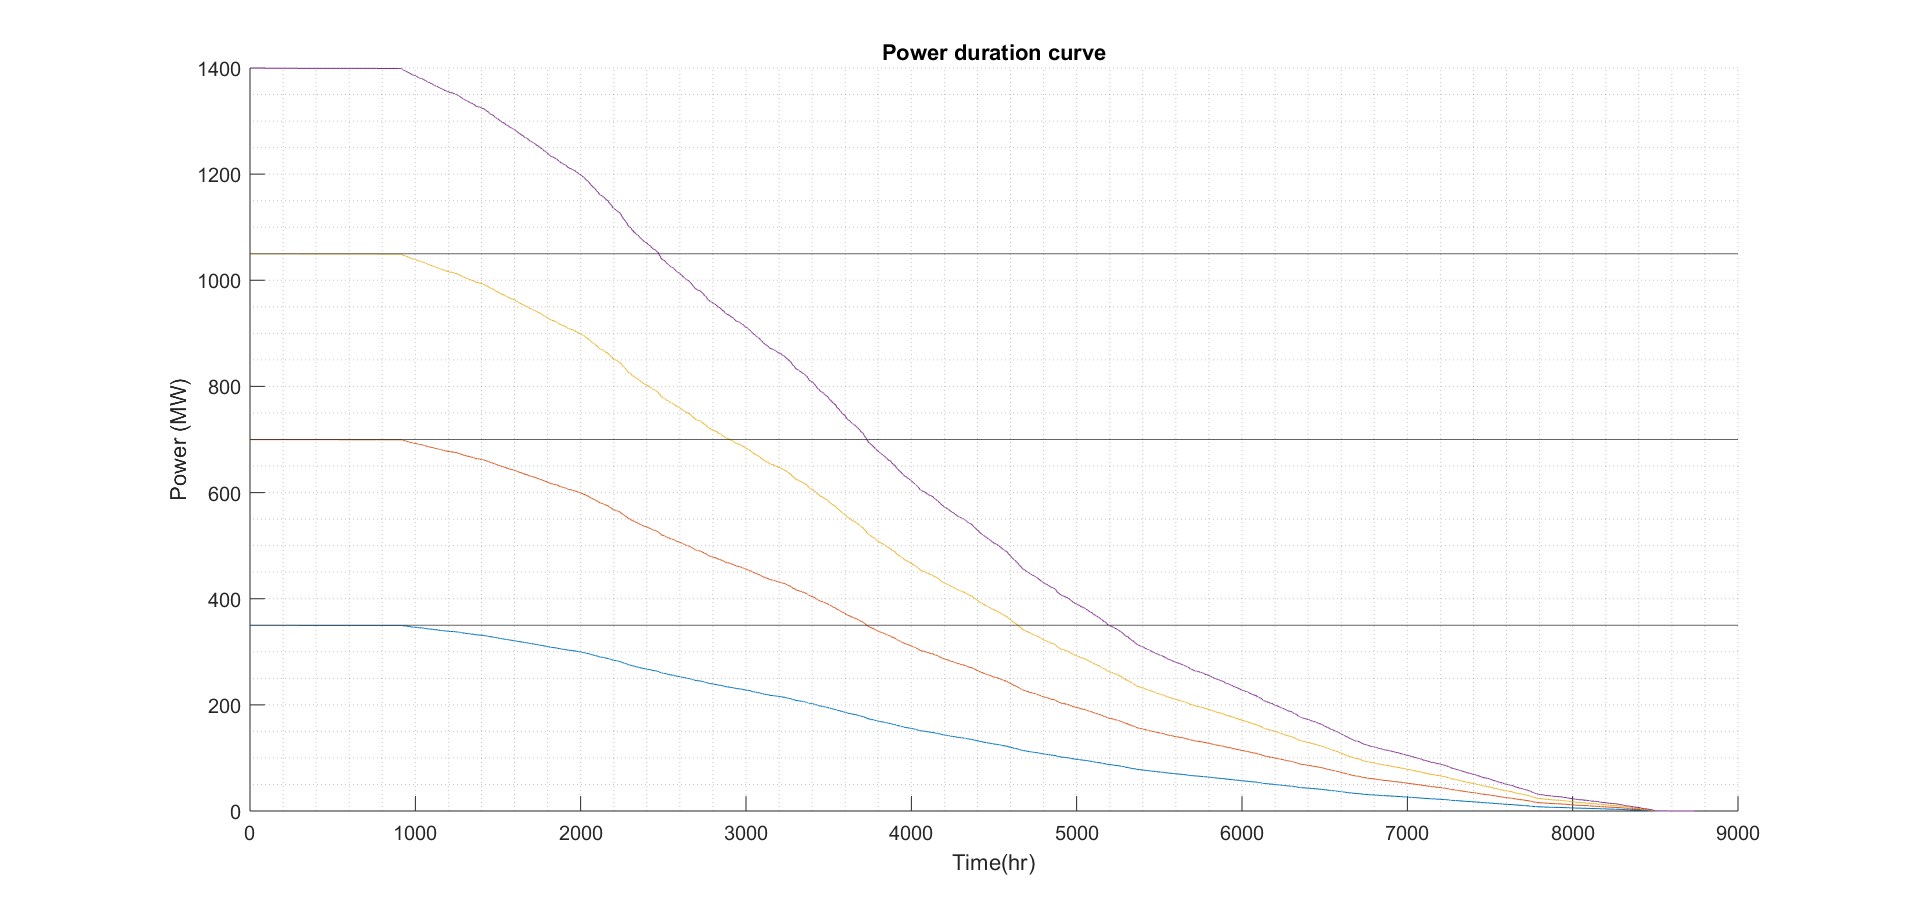
\includegraphics[width=0.8 \linewidth]{4_PDC.png}
        \caption{4 buses}
        \label{fig:couple}
\end{figure}
The decomposition model is used to find the probability when the coupler is attached. During this scenario all, the buses are in parallel with the coupler being in series,with a failure probability of 0.01. This induces a higher chance of failure with the combined probability of
0.069 and the energy lost is 37.8 GWh, which is  0.64\%.
%Omkar

\section*{\textbf{Exercise 8: revising the n-1 criterion}}

Redundancy means the duplication of critical components for preserving the continuity of supply. n-1 criteria says that the failure of a single component should not affect the operation of power system. However, implementing this criteria is not feasible for off-shore networks as the installation cost is substantial. Therefore it is beneficial to have more probabilistic redundancies t be adopted in the near future to tackle this situation.
Probabilistic approach is beneficial as it gives the provision to consider a large amount of factors for the reliability assessment. 

A power system with no redundancy is not an ideal situation as it poses a serious threat on the continuity of supply. Hence, some amount of redundancy must be implemented for off-shore networks. 

Reliability assessment is performed by evaluating the economic impact. There are many ways of implementing redundancies such as:
\begin{itemize}
    \item \textbf{Having a hub at sea configuration:}As it minimizes the probability of losing wind power due to some connection failure.
    \item Utilizing the on-shore generator spinning reserve.
    \item Installation of storage facilities.
    \item In extreme conditions, demand side management operations such as peak shaving can be performed.
  \end{itemize}
  
In the future, it is expected that there will  be large scale interconnection of offshore-onshore  networks for electricity trade. The failure of offshore network can adversely impact the reliability of onshore network.

When n-1 redundancy is applied to an onshore network with a double circuit , the maximal loading is about 55 percent. Assuming that the capacity of the cable is equal to that of generation, to increase the loading when one circuit fails; we can use  branch and hub couplers, especially when the distance to the shore is high.